\documentclass[1p]{elsarticle_modified}
%\bibliographystyle{elsarticle-num}

%\usepackage[colorlinks]{hyperref}
%\usepackage{abbrmath_seonhwa} %\Abb, \Ascr, \Acal ,\Abf, \Afrak
\usepackage{amsfonts}
\usepackage{amssymb}
\usepackage{amsmath}
\usepackage{amsthm}
\usepackage{scalefnt}
\usepackage{amsbsy}
\usepackage{kotex}
\usepackage{caption}
\usepackage{subfig}
\usepackage{color}
\usepackage{graphicx}
\usepackage{xcolor} %% white, black, red, green, blue, cyan, magenta, yellow
\usepackage{float}
\usepackage{setspace}
\usepackage{hyperref}

\usepackage{tikz}
\usetikzlibrary{arrows}

\usepackage{multirow}
\usepackage{array} % fixed length table
\usepackage{hhline}

%%%%%%%%%%%%%%%%%%%%%
\makeatletter
\renewcommand*\env@matrix[1][\arraystretch]{%
	\edef\arraystretch{#1}%
	\hskip -\arraycolsep
	\let\@ifnextchar\new@ifnextchar
	\array{*\c@MaxMatrixCols c}}
\makeatother %https://tex.stackexchange.com/questions/14071/how-can-i-increase-the-line-spacing-in-a-matrix
%%%%%%%%%%%%%%%

\usepackage[normalem]{ulem}

\newcommand{\msout}[1]{\ifmmode\text{\sout{\ensuremath{#1}}}\else\sout{#1}\fi}
%SOURCE: \msout is \stkout macro in https://tex.stackexchange.com/questions/20609/strikeout-in-math-mode

\newcommand{\cancel}[1]{
	\ifmmode
	{\color{red}\msout{#1}}
	\else
	{\color{red}\sout{#1}}
	\fi
}

\newcommand{\add}[1]{
	{\color{blue}\uwave{#1}}
}

\newcommand{\replace}[2]{
	\ifmmode
	{\color{red}\msout{#1}}{\color{blue}\uwave{#2}}
	\else
	{\color{red}\sout{#1}}{\color{blue}\uwave{#2}}
	\fi
}

\newcommand{\Sol}{\mathcal{S}} %segment
\newcommand{\D}{D} %diagram
\newcommand{\A}{\mathcal{A}} %arc


%%%%%%%%%%%%%%%%%%%%%%%%%%%%%5 test

\def\sl{\operatorname{\textup{SL}}(2,\Cbb)}
\def\psl{\operatorname{\textup{PSL}}(2,\Cbb)}
\def\quan{\mkern 1mu \triangleright \mkern 1mu}

\theoremstyle{definition}
\newtheorem{thm}{Theorem}[section]
\newtheorem{prop}[thm]{Proposition}
\newtheorem{lem}[thm]{Lemma}
\newtheorem{ques}[thm]{Question}
\newtheorem{cor}[thm]{Corollary}
\newtheorem{defn}[thm]{Definition}
\newtheorem{exam}[thm]{Example}
\newtheorem{rmk}[thm]{Remark}
\newtheorem{alg}[thm]{Algorithm}

\newcommand{\I}{\sqrt{-1}}
\begin{document}

%\begin{frontmatter}
%
%\title{Boundary parabolic representations of knots up to 8 crossings}
%
%%% Group authors per affiliation:
%\author{Yunhi Cho} 
%\address{Department of Mathematics, University of Seoul, Seoul, Korea}
%\ead{yhcho@uos.ac.kr}
%
%
%\author{Seonhwa Kim} %\fnref{s_kim}}
%\address{Center for Geometry and Physics, Institute for Basic Science, Pohang, 37673, Korea}
%\ead{ryeona17@ibs.re.kr}
%
%\author{Hyuk Kim}
%\address{Department of Mathematical Sciences, Seoul National University, Seoul 08826, Korea}
%\ead{hyukkim@snu.ac.kr}
%
%\author{Seokbeom Yoon}
%\address{Department of Mathematical Sciences, Seoul National University, Seoul, 08826,  Korea}
%\ead{sbyoon15@snu.ac.kr}
%
%\begin{abstract}
%We find all boundary parabolic representation of knots up to 8 crossings.
%
%\end{abstract}
%\begin{keyword}
%    \MSC[2010] 57M25 
%\end{keyword}
%
%\end{frontmatter}

%\linenumbers
%\tableofcontents
%
\newcommand\colored[1]{\textcolor{white}{\rule[-0.35ex]{0.8em}{1.4ex}}\kern-0.8em\color{red} #1}%
%\newcommand\colored[1]{\textcolor{white}{ #1}\kern-2.17ex	\textcolor{white}{ #1}\kern-1.81ex	\textcolor{white}{ #1}\kern-2.15ex\color{red}#1	}

{\Large $\underline{12a_{0315}~(K12a_{0315})}$}

\setlength{\tabcolsep}{10pt}
\renewcommand{\arraystretch}{1.6}
\vspace{1cm}\begin{tabular}{m{100pt}>{\centering\arraybackslash}m{274pt}}
\multirow{5}{120pt}{
	\centering
	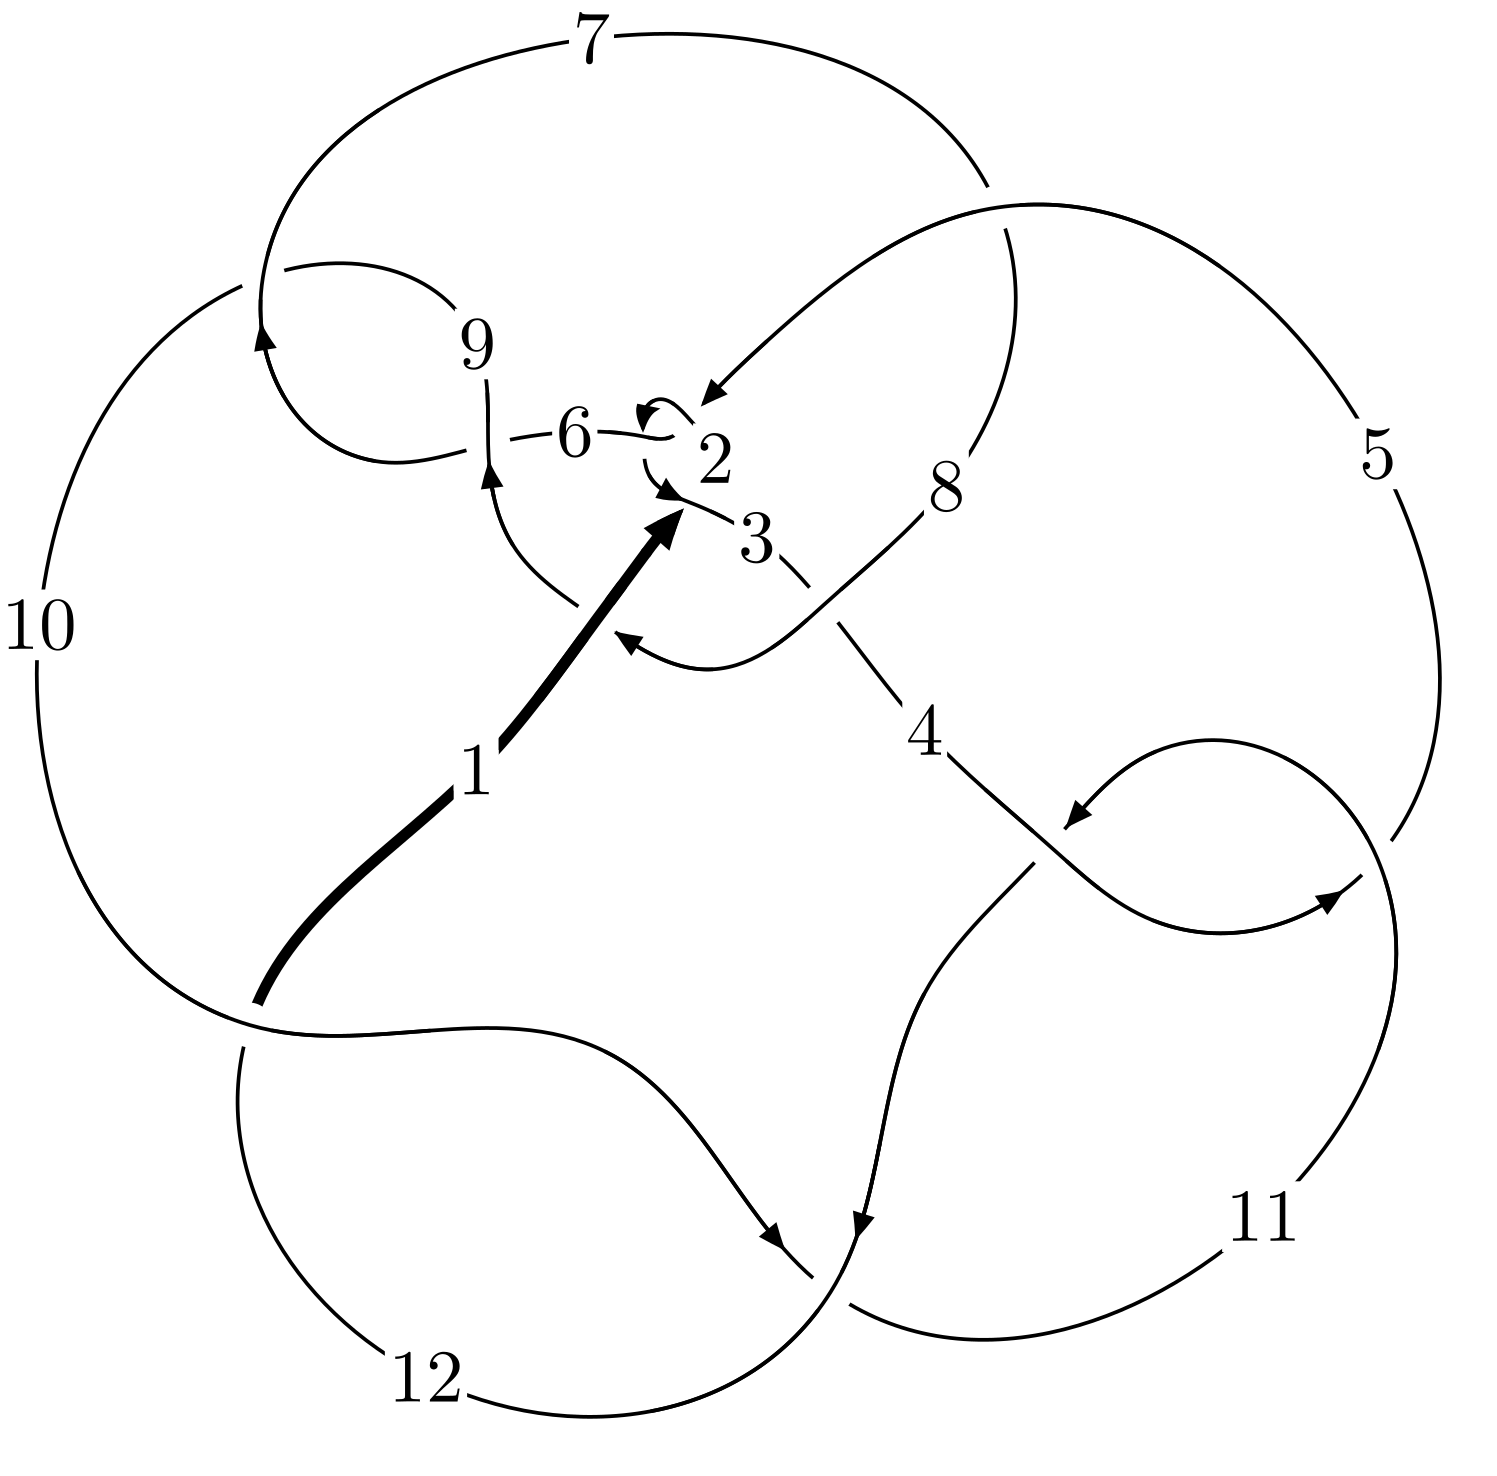
\includegraphics[width=112pt]{../../../GIT/diagram.site/Diagrams/png/1116_12a_0315.png}\\
\ \ \ A knot diagram\footnotemark}&
\allowdisplaybreaks
\textbf{Linearized knot diagam} \\
\cline{2-2}
 &
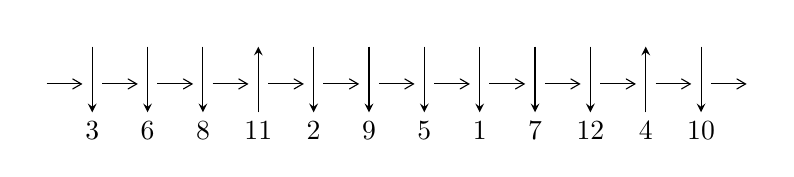
\begin{tikzpicture}[x=20pt, y=17pt]
	% nodes
	\node (C0) at (0, 0) {};
	\node (C1) at (1, 0) {};
	\node (C1U) at (1, +1) {};
	\node (C1D) at (1, -1) {3};

	\node (C2) at (2, 0) {};
	\node (C2U) at (2, +1) {};
	\node (C2D) at (2, -1) {6};

	\node (C3) at (3, 0) {};
	\node (C3U) at (3, +1) {};
	\node (C3D) at (3, -1) {8};

	\node (C4) at (4, 0) {};
	\node (C4U) at (4, +1) {};
	\node (C4D) at (4, -1) {11};

	\node (C5) at (5, 0) {};
	\node (C5U) at (5, +1) {};
	\node (C5D) at (5, -1) {2};

	\node (C6) at (6, 0) {};
	\node (C6U) at (6, +1) {};
	\node (C6D) at (6, -1) {9};

	\node (C7) at (7, 0) {};
	\node (C7U) at (7, +1) {};
	\node (C7D) at (7, -1) {5};

	\node (C8) at (8, 0) {};
	\node (C8U) at (8, +1) {};
	\node (C8D) at (8, -1) {1};

	\node (C9) at (9, 0) {};
	\node (C9U) at (9, +1) {};
	\node (C9D) at (9, -1) {7};

	\node (C10) at (10, 0) {};
	\node (C10U) at (10, +1) {};
	\node (C10D) at (10, -1) {12};

	\node (C11) at (11, 0) {};
	\node (C11U) at (11, +1) {};
	\node (C11D) at (11, -1) {4};

	\node (C12) at (12, 0) {};
	\node (C12U) at (12, +1) {};
	\node (C12D) at (12, -1) {10};
	\node (C13) at (13, 0) {};

	% arrows
	\draw[->,>={angle 60}]
	(C0) edge (C1) (C1) edge (C2) (C2) edge (C3) (C3) edge (C4) (C4) edge (C5) (C5) edge (C6) (C6) edge (C7) (C7) edge (C8) (C8) edge (C9) (C9) edge (C10) (C10) edge (C11) (C11) edge (C12) (C12) edge (C13) ;	\draw[->,>=stealth]
	(C1U) edge (C1D) (C2U) edge (C2D) (C3U) edge (C3D) (C4D) edge (C4U) (C5U) edge (C5D) (C6U) edge (C6D) (C7U) edge (C7D) (C8U) edge (C8D) (C9U) edge (C9D) (C10U) edge (C10D) (C11D) edge (C11U) (C12U) edge (C12D) ;
	\end{tikzpicture} \\
\hhline{~~} \\& 
\textbf{Solving Sequence} \\ \cline{2-2} 
 &
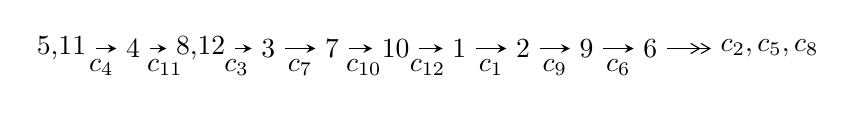
\begin{tikzpicture}[x=23pt, y=7pt]
	% node
	\node (A0) at (-1/8, 0) {5,11};
	\node (A1) at (1, 0) {4};
	\node (A2) at (33/16, 0) {8,12};
	\node (A3) at (25/8, 0) {3};
	\node (A4) at (33/8, 0) {7};
	\node (A5) at (41/8, 0) {10};
	\node (A6) at (49/8, 0) {1};
	\node (A7) at (57/8, 0) {2};
	\node (A8) at (65/8, 0) {9};
	\node (A9) at (73/8, 0) {6};
	\node (C1) at (1/2, -1) {$c_{4}$};
	\node (C2) at (3/2, -1) {$c_{11}$};
	\node (C3) at (21/8, -1) {$c_{3}$};
	\node (C4) at (29/8, -1) {$c_{7}$};
	\node (C5) at (37/8, -1) {$c_{10}$};
	\node (C6) at (45/8, -1) {$c_{12}$};
	\node (C7) at (53/8, -1) {$c_{1}$};
	\node (C8) at (61/8, -1) {$c_{9}$};
	\node (C9) at (69/8, -1) {$c_{6}$};
	\node (A10) at (11, 0) {$c_{2},c_{5},c_{8}$};

	% edge
	\draw[->,>=stealth]	
	(A0) edge (A1) (A1) edge (A2) (A2) edge (A3) (A3) edge (A4) (A4) edge (A5) (A5) edge (A6) (A6) edge (A7) (A7) edge (A8) (A8) edge (A9) ;
	\draw[->>,>={angle 60}]	
	(A9) edge (A10);
\end{tikzpicture} \\ 

\end{tabular} \\

\footnotetext{
The image of knot diagram is generated by the software ``\textbf{Draw programme}" developed by Andrew Bartholomew(\url{http://www.layer8.co.uk/maths/draw/index.htm\#Running-draw}), where we modified some parts for our purpose(\url{https://github.com/CATsTAILs/LinksPainter}).
}\phantom \\ \newline 
\centering \textbf{Ideals for irreducible components\footnotemark of $X_{\text{par}}$} 
 
\begin{align*}
I^u_{1}&=\langle 
-1.85167\times10^{121} u^{114}-3.72449\times10^{121} u^{113}+\cdots+7.44095\times10^{121} b+3.07946\times10^{121},\\
\phantom{I^u_{1}}&\phantom{= \langle  }-5.89851\times10^{121} u^{114}-8.95585\times10^{121} u^{113}+\cdots+7.44095\times10^{121} a-1.95302\times10^{122},\\
\phantom{I^u_{1}}&\phantom{= \langle  }u^{115}+2 u^{114}+\cdots+2 u-1\rangle \\
I^u_{2}&=\langle 
3 u^4+4 u^3+5 u^2+5 b+u,\;- u^4- u^3+u^2+5 a+3 u+4,\;u^5+u^4+2 u^3+u^2+u+1\rangle \\
\\
\end{align*}
\raggedright * 2 irreducible components of $\dim_{\mathbb{C}}=0$, with total 120 representations.\\
\footnotetext{All coefficients of polynomials are rational numbers. But the coefficients are sometimes approximated in decimal forms when there is not enough margin.}
\newpage
\renewcommand{\arraystretch}{1}
\centering \section*{I. $I^u_{1}= \langle -1.85\times10^{121} u^{114}-3.72\times10^{121} u^{113}+\cdots+7.44\times10^{121} b+3.08\times10^{121},\;-5.90\times10^{121} u^{114}-8.96\times10^{121} u^{113}+\cdots+7.44\times10^{121} a-1.95\times10^{122},\;u^{115}+2 u^{114}+\cdots+2 u-1 \rangle$}
\flushleft \textbf{(i) Arc colorings}\\
\begin{tabular}{m{7pt} m{180pt} m{7pt} m{180pt} }
\flushright $a_{5}=$&$\begin{pmatrix}1\\0\end{pmatrix}$ \\
\flushright $a_{11}=$&$\begin{pmatrix}0\\u\end{pmatrix}$ \\
\flushright $a_{4}=$&$\begin{pmatrix}1\\u^2\end{pmatrix}$ \\
\flushright $a_{8}=$&$\begin{pmatrix}0.792709 u^{114}+1.20359 u^{113}+\cdots-4.75680 u+2.62469\\0.248849 u^{114}+0.500539 u^{113}+\cdots+3.03902 u-0.413853\end{pmatrix}$ \\
\flushright $a_{12}=$&$\begin{pmatrix}u\\u^3+u\end{pmatrix}$ \\
\flushright $a_{3}=$&$\begin{pmatrix}1.62371 u^{114}+2.67004 u^{113}+\cdots-3.94611 u+0.349188\\-0.816496 u^{114}-1.64935 u^{113}+\cdots+1.57453 u-0.0503323\end{pmatrix}$ \\
\flushright $a_{7}=$&$\begin{pmatrix}1.04156 u^{114}+1.70413 u^{113}+\cdots-1.71778 u+2.21083\\0.248849 u^{114}+0.500539 u^{113}+\cdots+3.03902 u-0.413853\end{pmatrix}$ \\
\flushright $a_{10}=$&$\begin{pmatrix}u^3\\u^5+u^3+u\end{pmatrix}$ \\
\flushright $a_{1}=$&$\begin{pmatrix}u^5+u\\u^7+u^5+2 u^3+u\end{pmatrix}$ \\
\flushright $a_{2}=$&$\begin{pmatrix}-0.495778 u^{114}+0.152549 u^{113}+\cdots+2.54880 u-1.59091\\0.430896 u^{114}+0.364813 u^{113}+\cdots-0.748946 u+0.656296\end{pmatrix}$ \\
\flushright $a_{9}=$&$\begin{pmatrix}1.35088 u^{114}+2.29904 u^{113}+\cdots-4.32285 u+2.45638\\0.219430 u^{114}+0.633152 u^{113}+\cdots+4.57775 u-0.762711\end{pmatrix}$ \\
\flushright $a_{6}=$&$\begin{pmatrix}-0.580563 u^{114}-1.39437 u^{113}+\cdots+4.59835 u-0.240154\\-0.143312 u^{114}-0.582118 u^{113}+\cdots-1.63332 u+0.499825\end{pmatrix}$\\&\end{tabular}
\flushleft \textbf{(ii) Obstruction class $= -1$}\\~\\
\flushleft \textbf{(iii) Cusp Shapes $= -5.26127 u^{114}-13.4625 u^{113}+\cdots-1.05644 u-6.56776$}\\~\\
\newpage\renewcommand{\arraystretch}{1}
\flushleft \textbf{(iv) u-Polynomials at the component}\newline \\
\begin{tabular}{m{50pt}|m{274pt}}
Crossings & \hspace{64pt}u-Polynomials at each crossing \\
\hline $$\begin{aligned}c_{1}\end{aligned}$$&$\begin{aligned}
&u^{115}+52 u^{114}+\cdots+8 u+1
\end{aligned}$\\
\hline $$\begin{aligned}c_{2},c_{5}\end{aligned}$$&$\begin{aligned}
&u^{115}+2 u^{114}+\cdots+4 u+1
\end{aligned}$\\
\hline $$\begin{aligned}c_{3}\end{aligned}$$&$\begin{aligned}
&u^{115}+u^{114}+\cdots-4000 u+20000
\end{aligned}$\\
\hline $$\begin{aligned}c_{4},c_{11}\end{aligned}$$&$\begin{aligned}
&u^{115}-2 u^{114}+\cdots+2 u+1
\end{aligned}$\\
\hline $$\begin{aligned}c_{6},c_{9}\end{aligned}$$&$\begin{aligned}
&u^{115}-6 u^{114}+\cdots-6050 u+625
\end{aligned}$\\
\hline $$\begin{aligned}c_{7}\end{aligned}$$&$\begin{aligned}
&25(25 u^{115}+1297 u^{113}+\cdots-6356084 u+531211)
\end{aligned}$\\
\hline $$\begin{aligned}c_{8}\end{aligned}$$&$\begin{aligned}
&25(25 u^{115}+25 u^{114}+\cdots+165472 u+46912)
\end{aligned}$\\
\hline $$\begin{aligned}c_{10},c_{12}\end{aligned}$$&$\begin{aligned}
&u^{115}+36 u^{114}+\cdots+8 u-1
\end{aligned}$\\
\hline
\end{tabular}\\~\\
\newpage\renewcommand{\arraystretch}{1}
\flushleft \textbf{(v) Riley Polynomials at the component}\newline \\
\begin{tabular}{m{50pt}|m{274pt}}
Crossings & \hspace{64pt}Riley Polynomials at each crossing \\
\hline $$\begin{aligned}c_{1}\end{aligned}$$&$\begin{aligned}
&y^{115}+24 y^{114}+\cdots-4 y-1
\end{aligned}$\\
\hline $$\begin{aligned}c_{2},c_{5}\end{aligned}$$&$\begin{aligned}
&y^{115}-52 y^{114}+\cdots+8 y-1
\end{aligned}$\\
\hline $$\begin{aligned}c_{3}\end{aligned}$$&$\begin{aligned}
&y^{115}+33 y^{114}+\cdots+2280000000 y-400000000
\end{aligned}$\\
\hline $$\begin{aligned}c_{4},c_{11}\end{aligned}$$&$\begin{aligned}
&y^{115}+36 y^{114}+\cdots+8 y-1
\end{aligned}$\\
\hline $$\begin{aligned}c_{6},c_{9}\end{aligned}$$&$\begin{aligned}
&y^{115}-64 y^{114}+\cdots-9508750 y-390625
\end{aligned}$\\
\hline $$\begin{aligned}c_{7}\end{aligned}$$&$\begin{aligned}
&625\\
&\cdot(625 y^{115}+64850 y^{114}+\cdots+4263135428918 y-282185126521)
\end{aligned}$\\
\hline $$\begin{aligned}c_{8}\end{aligned}$$&$\begin{aligned}
&625(625 y^{115}-37225 y^{114}+\cdots-4.94556\times10^{10} y-2.20074\times10^{9})
\end{aligned}$\\
\hline $$\begin{aligned}c_{10},c_{12}\end{aligned}$$&$\begin{aligned}
&y^{115}+88 y^{114}+\cdots+180 y-1
\end{aligned}$\\
\hline
\end{tabular}\\~\\
\newpage\flushleft \textbf{(vi) Complex Volumes and Cusp Shapes}
$$\begin{array}{c|c|c}  
\text{Solutions to }I^u_{1}& \I (\text{vol} + \sqrt{-1}CS) & \text{Cusp shape}\\
 \hline 
\begin{aligned}
u &= \phantom{-}0.231824 + 0.953832 I \\
a &= -2.46206 + 0.91607 I \\
b &= \phantom{-}0.596166 - 0.796359 I\end{aligned}
 & -0.78095 + 7.32794 I & \phantom{-0.000000 } 0 \\ \hline\begin{aligned}
u &= \phantom{-}0.231824 - 0.953832 I \\
a &= -2.46206 - 0.91607 I \\
b &= \phantom{-}0.596166 + 0.796359 I\end{aligned}
 & -0.78095 - 7.32794 I & \phantom{-0.000000 } 0 \\ \hline\begin{aligned}
u &= -0.262847 + 0.932497 I \\
a &= \phantom{-}1.91342 + 0.84423 I \\
b &= -0.370130 - 0.643087 I\end{aligned}
 & \phantom{-}0.61191 - 2.36422 I & \phantom{-0.000000 } 0 \\ \hline\begin{aligned}
u &= -0.262847 - 0.932497 I \\
a &= \phantom{-}1.91342 - 0.84423 I \\
b &= -0.370130 + 0.643087 I\end{aligned}
 & \phantom{-}0.61191 + 2.36422 I & \phantom{-0.000000 } 0 \\ \hline\begin{aligned}
u &= \phantom{-}0.719284 + 0.761224 I \\
a &= -0.455850 - 1.230130 I \\
b &= -0.384714 - 0.124611 I\end{aligned}
 & -0.13012 - 4.17483 I & \phantom{-0.000000 } 0 \\ \hline\begin{aligned}
u &= \phantom{-}0.719284 - 0.761224 I \\
a &= -0.455850 + 1.230130 I \\
b &= -0.384714 + 0.124611 I\end{aligned}
 & -0.13012 + 4.17483 I & \phantom{-0.000000 } 0 \\ \hline\begin{aligned}
u &= \phantom{-}0.679610 + 0.799058 I \\
a &= -1.17140 - 1.41956 I \\
b &= \phantom{-}0.495600 - 0.123968 I\end{aligned}
 & -1.60723 + 1.91504 I & \phantom{-0.000000 } 0 \\ \hline\begin{aligned}
u &= \phantom{-}0.679610 - 0.799058 I \\
a &= -1.17140 + 1.41956 I \\
b &= \phantom{-}0.495600 + 0.123968 I\end{aligned}
 & -1.60723 - 1.91504 I & \phantom{-0.000000 } 0 \\ \hline\begin{aligned}
u &= -0.082837 + 0.941587 I \\
a &= \phantom{-}2.46261 - 1.38632 I \\
b &= -0.990156 - 0.172748 I\end{aligned}
 & -5.35130 - 4.97918 I & \phantom{-0.000000 } 0 \\ \hline\begin{aligned}
u &= -0.082837 - 0.941587 I \\
a &= \phantom{-}2.46261 + 1.38632 I \\
b &= -0.990156 + 0.172748 I\end{aligned}
 & -5.35130 + 4.97918 I & \phantom{-0.000000 } 0\\
 \hline 
 \end{array}$$\newpage$$\begin{array}{c|c|c}  
\text{Solutions to }I^u_{1}& \I (\text{vol} + \sqrt{-1}CS) & \text{Cusp shape}\\
 \hline 
\begin{aligned}
u &= -0.814912 + 0.678676 I \\
a &= -0.199202 + 0.199306 I \\
b &= \phantom{-}0.110561 + 1.268530 I\end{aligned}
 & \phantom{-}4.77410 - 2.66895 I & \phantom{-0.000000 } 0 \\ \hline\begin{aligned}
u &= -0.814912 - 0.678676 I \\
a &= -0.199202 - 0.199306 I \\
b &= \phantom{-}0.110561 - 1.268530 I\end{aligned}
 & \phantom{-}4.77410 + 2.66895 I & \phantom{-0.000000 } 0 \\ \hline\begin{aligned}
u &= -0.031070 + 0.935882 I \\
a &= \phantom{-}1.05114 - 1.63997 I \\
b &= -0.443506 - 0.129637 I\end{aligned}
 & -6.14284 + 1.16940 I & \phantom{-0.000000 } 0 \\ \hline\begin{aligned}
u &= -0.031070 - 0.935882 I \\
a &= \phantom{-}1.05114 + 1.63997 I \\
b &= -0.443506 + 0.129637 I\end{aligned}
 & -6.14284 - 1.16940 I & \phantom{-0.000000 } 0 \\ \hline\begin{aligned}
u &= -0.646217 + 0.859121 I \\
a &= \phantom{-}1.74516 - 1.15528 I \\
b &= -1.208750 + 0.062952 I\end{aligned}
 & -2.57690 + 0.59772 I & \phantom{-0.000000 } 0 \\ \hline\begin{aligned}
u &= -0.646217 - 0.859121 I \\
a &= \phantom{-}1.74516 + 1.15528 I \\
b &= -1.208750 - 0.062952 I\end{aligned}
 & -2.57690 - 0.59772 I & \phantom{-0.000000 } 0 \\ \hline\begin{aligned}
u &= -0.732062 + 0.787501 I \\
a &= \phantom{-}0.687215 - 0.808553 I \\
b &= \phantom{-}0.329674 - 0.594451 I\end{aligned}
 & \phantom{-}1.59979 - 0.04409 I & \phantom{-0.000000 } 0 \\ \hline\begin{aligned}
u &= -0.732062 - 0.787501 I \\
a &= \phantom{-}0.687215 + 0.808553 I \\
b &= \phantom{-}0.329674 + 0.594451 I\end{aligned}
 & \phantom{-}1.59979 + 0.04409 I & \phantom{-0.000000 } 0 \\ \hline\begin{aligned}
u &= -0.099706 + 1.078560 I \\
a &= -0.48505 - 1.37837 I \\
b &= \phantom{-}0.203969 + 0.981425 I\end{aligned}
 & -0.66867 - 2.87209 I & \phantom{-0.000000 } 0 \\ \hline\begin{aligned}
u &= -0.099706 - 1.078560 I \\
a &= -0.48505 + 1.37837 I \\
b &= \phantom{-}0.203969 - 0.981425 I\end{aligned}
 & -0.66867 + 2.87209 I & \phantom{-0.000000 } 0\\
 \hline 
 \end{array}$$\newpage$$\begin{array}{c|c|c}  
\text{Solutions to }I^u_{1}& \I (\text{vol} + \sqrt{-1}CS) & \text{Cusp shape}\\
 \hline 
\begin{aligned}
u &= \phantom{-}0.156085 + 0.900887 I \\
a &= -2.53802 - 0.37596 I \\
b &= \phantom{-}0.966548 - 0.328199 I\end{aligned}
 & -3.59301 + 1.68133 I & \phantom{-0.000000 } 0 \\ \hline\begin{aligned}
u &= \phantom{-}0.156085 - 0.900887 I \\
a &= -2.53802 + 0.37596 I \\
b &= \phantom{-}0.966548 + 0.328199 I\end{aligned}
 & -3.59301 - 1.68133 I & \phantom{-0.000000 } 0 \\ \hline\begin{aligned}
u &= \phantom{-}0.846369 + 0.687021 I \\
a &= \phantom{-}0.202537 + 0.074386 I \\
b &= \phantom{-}0.247444 + 1.370760 I\end{aligned}
 & \phantom{-}5.98557 - 3.08518 I & \phantom{-0.000000 } 0 \\ \hline\begin{aligned}
u &= \phantom{-}0.846369 - 0.687021 I \\
a &= \phantom{-}0.202537 - 0.074386 I \\
b &= \phantom{-}0.247444 - 1.370760 I\end{aligned}
 & \phantom{-}5.98557 + 3.08518 I & \phantom{-0.000000 } 0 \\ \hline\begin{aligned}
u &= \phantom{-}0.120992 + 0.896882 I \\
a &= -0.30902 - 1.97202 I \\
b &= \phantom{-}0.286071 + 1.066620 I\end{aligned}
 & -1.07660 - 2.43604 I & \phantom{-0.000000 } 0 \\ \hline\begin{aligned}
u &= \phantom{-}0.120992 - 0.896882 I \\
a &= -0.30902 + 1.97202 I \\
b &= \phantom{-}0.286071 - 1.066620 I\end{aligned}
 & -1.07660 + 2.43604 I & \phantom{-0.000000 } 0 \\ \hline\begin{aligned}
u &= \phantom{-}0.078739 + 0.893461 I \\
a &= -2.18286 - 0.57596 I \\
b &= \phantom{-}0.992060 - 0.472687 I\end{aligned}
 & -3.51720 + 1.23198 I & \phantom{-0.000000 } 0 \\ \hline\begin{aligned}
u &= \phantom{-}0.078739 - 0.893461 I \\
a &= -2.18286 + 0.57596 I \\
b &= \phantom{-}0.992060 + 0.472687 I\end{aligned}
 & -3.51720 - 1.23198 I & \phantom{-0.000000 } 0 \\ \hline\begin{aligned}
u &= \phantom{-}0.683059 + 0.873025 I \\
a &= -1.12060 - 1.09313 I \\
b &= \phantom{-}1.48924 + 0.10894 I\end{aligned}
 & -0.36733 + 2.63401 I & \phantom{-0.000000 } 0 \\ \hline\begin{aligned}
u &= \phantom{-}0.683059 - 0.873025 I \\
a &= -1.12060 + 1.09313 I \\
b &= \phantom{-}1.48924 - 0.10894 I\end{aligned}
 & -0.36733 - 2.63401 I & \phantom{-0.000000 } 0\\
 \hline 
 \end{array}$$\newpage$$\begin{array}{c|c|c}  
\text{Solutions to }I^u_{1}& \I (\text{vol} + \sqrt{-1}CS) & \text{Cusp shape}\\
 \hline 
\begin{aligned}
u &= \phantom{-}0.870156 + 0.172696 I \\
a &= -0.0912549 - 0.0114818 I \\
b &= -0.438004 + 0.516951 I\end{aligned}
 & -4.21088 + 0.70500 I & \phantom{-0.000000 } 0 \\ \hline\begin{aligned}
u &= \phantom{-}0.870156 - 0.172696 I \\
a &= -0.0912549 + 0.0114818 I \\
b &= -0.438004 - 0.516951 I\end{aligned}
 & -4.21088 - 0.70500 I & \phantom{-0.000000 } 0 \\ \hline\begin{aligned}
u &= -0.659858 + 0.899578 I \\
a &= \phantom{-}1.52640 - 0.24867 I \\
b &= -1.090120 + 0.070208 I\end{aligned}
 & -2.72537 - 5.66569 I & \phantom{-0.000000 } 0 \\ \hline\begin{aligned}
u &= -0.659858 - 0.899578 I \\
a &= \phantom{-}1.52640 + 0.24867 I \\
b &= -1.090120 - 0.070208 I\end{aligned}
 & -2.72537 + 5.66569 I & \phantom{-0.000000 } 0 \\ \hline\begin{aligned}
u &= -0.749840 + 0.829632 I \\
a &= \phantom{-}1.350280 + 0.409157 I \\
b &= \phantom{-}1.01467 - 1.70820 I\end{aligned}
 & \phantom{-}2.33638 - 0.47130 I & \phantom{-0.000000 } 0 \\ \hline\begin{aligned}
u &= -0.749840 - 0.829632 I \\
a &= \phantom{-}1.350280 - 0.409157 I \\
b &= \phantom{-}1.01467 + 1.70820 I\end{aligned}
 & \phantom{-}2.33638 + 0.47130 I & \phantom{-0.000000 } 0 \\ \hline\begin{aligned}
u &= -0.822875 + 0.764427 I \\
a &= -0.391586 + 0.012215 I \\
b &= \phantom{-}0.88291 - 1.12333 I\end{aligned}
 & \phantom{-}5.95773 + 6.05581 I & \phantom{-0.000000 } 0 \\ \hline\begin{aligned}
u &= -0.822875 - 0.764427 I \\
a &= -0.391586 - 0.012215 I \\
b &= \phantom{-}0.88291 + 1.12333 I\end{aligned}
 & \phantom{-}5.95773 - 6.05581 I & \phantom{-0.000000 } 0 \\ \hline\begin{aligned}
u &= -0.791646 + 0.800114 I \\
a &= \phantom{-}0.0681291 - 0.0048683 I \\
b &= \phantom{-}0.807966 - 0.785235 I\end{aligned}
 & \phantom{-}2.31006 + 0.02277 I & \phantom{-0.000000 } 0 \\ \hline\begin{aligned}
u &= -0.791646 - 0.800114 I \\
a &= \phantom{-}0.0681291 + 0.0048683 I \\
b &= \phantom{-}0.807966 + 0.785235 I\end{aligned}
 & \phantom{-}2.31006 - 0.02277 I & \phantom{-0.000000 } 0\\
 \hline 
 \end{array}$$\newpage$$\begin{array}{c|c|c}  
\text{Solutions to }I^u_{1}& \I (\text{vol} + \sqrt{-1}CS) & \text{Cusp shape}\\
 \hline 
\begin{aligned}
u &= \phantom{-}0.877305 + 0.708965 I \\
a &= \phantom{-}0.125553 - 0.108050 I \\
b &= \phantom{-}0.94576 + 1.42038 I\end{aligned}
 & \phantom{-}4.88341 - 7.17921 I & \phantom{-0.000000 } 0 \\ \hline\begin{aligned}
u &= \phantom{-}0.877305 - 0.708965 I \\
a &= \phantom{-}0.125553 + 0.108050 I \\
b &= \phantom{-}0.94576 - 1.42038 I\end{aligned}
 & \phantom{-}4.88341 + 7.17921 I & \phantom{-0.000000 } 0 \\ \hline\begin{aligned}
u &= -0.889873 + 0.693456 I \\
a &= -0.0644567 - 0.0226712 I \\
b &= -0.802417 + 1.025230 I\end{aligned}
 & -1.07673 + 4.48539 I & \phantom{-0.000000 } 0 \\ \hline\begin{aligned}
u &= -0.889873 - 0.693456 I \\
a &= -0.0644567 + 0.0226712 I \\
b &= -0.802417 - 1.025230 I\end{aligned}
 & -1.07673 - 4.48539 I & \phantom{-0.000000 } 0 \\ \hline\begin{aligned}
u &= \phantom{-}0.747735 + 0.848567 I \\
a &= -3.17279 + 1.04812 I \\
b &= -1.29640 - 4.15597 I\end{aligned}
 & \phantom{-}1.68826 + 4.75505 I & \phantom{-0.000000 } 0 \\ \hline\begin{aligned}
u &= \phantom{-}0.747735 - 0.848567 I \\
a &= -3.17279 - 1.04812 I \\
b &= -1.29640 + 4.15597 I\end{aligned}
 & \phantom{-}1.68826 - 4.75505 I & \phantom{-0.000000 } 0 \\ \hline\begin{aligned}
u &= \phantom{-}0.241160 + 1.108160 I \\
a &= \phantom{-}2.16055 - 0.75457 I \\
b &= -1.16119 + 0.96512 I\end{aligned}
 & -4.80644 + 12.94150 I & \phantom{-0.000000 } 0 \\ \hline\begin{aligned}
u &= \phantom{-}0.241160 - 1.108160 I \\
a &= \phantom{-}2.16055 + 0.75457 I \\
b &= -1.16119 - 0.96512 I\end{aligned}
 & -4.80644 - 12.94150 I & \phantom{-0.000000 } 0 \\ \hline\begin{aligned}
u &= -0.227858 + 1.111020 I \\
a &= -1.84536 - 0.85683 I \\
b &= \phantom{-}0.979988 + 0.954915 I\end{aligned}
 & -2.58436 - 7.22243 I & \phantom{-0.000000 } 0 \\ \hline\begin{aligned}
u &= -0.227858 - 1.111020 I \\
a &= -1.84536 + 0.85683 I \\
b &= \phantom{-}0.979988 - 0.954915 I\end{aligned}
 & -2.58436 + 7.22243 I & \phantom{-0.000000 } 0\\
 \hline 
 \end{array}$$\newpage$$\begin{array}{c|c|c}  
\text{Solutions to }I^u_{1}& \I (\text{vol} + \sqrt{-1}CS) & \text{Cusp shape}\\
 \hline 
\begin{aligned}
u &= \phantom{-}0.829120 + 0.774149 I \\
a &= \phantom{-}0.315506 + 0.088053 I \\
b &= -0.732646 - 1.094480 I\end{aligned}
 & \phantom{-}7.49710 - 0.85393 I & \phantom{-0.000000 } 0 \\ \hline\begin{aligned}
u &= \phantom{-}0.829120 - 0.774149 I \\
a &= \phantom{-}0.315506 - 0.088053 I \\
b &= -0.732646 + 1.094480 I\end{aligned}
 & \phantom{-}7.49710 + 0.85393 I & \phantom{-0.000000 } 0 \\ \hline\begin{aligned}
u &= -0.881740 + 0.714170 I \\
a &= -0.090486 - 0.148849 I \\
b &= -1.14088 + 1.41196 I\end{aligned}
 & \phantom{-}2.75920 + 12.82710 I & \phantom{-0.000000 } 0 \\ \hline\begin{aligned}
u &= -0.881740 - 0.714170 I \\
a &= -0.090486 + 0.148849 I \\
b &= -1.14088 - 1.41196 I\end{aligned}
 & \phantom{-}2.75920 - 12.82710 I & \phantom{-0.000000 } 0 \\ \hline\begin{aligned}
u &= \phantom{-}0.688094 + 0.929601 I \\
a &= -0.419814 + 0.892789 I \\
b &= \phantom{-}0.265970 + 0.325650 I\end{aligned}
 & -2.01818 + 3.37967 I & \phantom{-0.000000 } 0 \\ \hline\begin{aligned}
u &= \phantom{-}0.688094 - 0.929601 I \\
a &= -0.419814 - 0.892789 I \\
b &= \phantom{-}0.265970 - 0.325650 I\end{aligned}
 & -2.01818 - 3.37967 I & \phantom{-0.000000 } 0 \\ \hline\begin{aligned}
u &= \phantom{-}0.351802 + 1.104650 I \\
a &= \phantom{-}0.31481 + 1.42375 I \\
b &= -0.747838 - 0.529760 I\end{aligned}
 & -4.15815 - 5.61157 I & \phantom{-0.000000 } 0 \\ \hline\begin{aligned}
u &= \phantom{-}0.351802 - 1.104650 I \\
a &= \phantom{-}0.31481 - 1.42375 I \\
b &= -0.747838 + 0.529760 I\end{aligned}
 & -4.15815 + 5.61157 I & \phantom{-0.000000 } 0 \\ \hline\begin{aligned}
u &= \phantom{-}0.739725 + 0.897296 I \\
a &= \phantom{-}4.36688 + 0.96638 I \\
b &= -2.03502 + 5.62532 I\end{aligned}
 & \phantom{-}1.53888 + 0.89181 I & \phantom{-0.000000 } 0 \\ \hline\begin{aligned}
u &= \phantom{-}0.739725 - 0.897296 I \\
a &= \phantom{-}4.36688 - 0.96638 I \\
b &= -2.03502 - 5.62532 I\end{aligned}
 & \phantom{-}1.53888 - 0.89181 I & \phantom{-0.000000 } 0\\
 \hline 
 \end{array}$$\newpage$$\begin{array}{c|c|c}  
\text{Solutions to }I^u_{1}& \I (\text{vol} + \sqrt{-1}CS) & \text{Cusp shape}\\
 \hline 
\begin{aligned}
u &= -0.395665 + 1.097030 I \\
a &= \phantom{-}0.017649 + 1.133270 I \\
b &= \phantom{-}0.550820 - 0.485400 I\end{aligned}
 & -1.63066 - 0.10437 I & \phantom{-0.000000 } 0 \\ \hline\begin{aligned}
u &= -0.395665 - 1.097030 I \\
a &= \phantom{-}0.017649 - 1.133270 I \\
b &= \phantom{-}0.550820 + 0.485400 I\end{aligned}
 & -1.63066 + 0.10437 I & \phantom{-0.000000 } 0 \\ \hline\begin{aligned}
u &= \phantom{-}0.852961 + 0.805684 I \\
a &= \phantom{-}0.189912 + 0.218450 I \\
b &= -0.369955 - 0.833667 I\end{aligned}
 & \phantom{-}6.76805 + 1.81713 I & \phantom{-0.000000 } 0 \\ \hline\begin{aligned}
u &= \phantom{-}0.852961 - 0.805684 I \\
a &= \phantom{-}0.189912 - 0.218450 I \\
b &= -0.369955 + 0.833667 I\end{aligned}
 & \phantom{-}6.76805 - 1.81713 I & \phantom{-0.000000 } 0 \\ \hline\begin{aligned}
u &= -0.736891 + 0.914102 I \\
a &= -1.71511 + 1.24495 I \\
b &= \phantom{-}1.53035 + 2.03390 I\end{aligned}
 & \phantom{-}2.07779 - 5.17426 I & \phantom{-0.000000 } 0 \\ \hline\begin{aligned}
u &= -0.736891 - 0.914102 I \\
a &= -1.71511 - 1.24495 I \\
b &= \phantom{-}1.53035 - 2.03390 I\end{aligned}
 & \phantom{-}2.07779 + 5.17426 I & \phantom{-0.000000 } 0 \\ \hline\begin{aligned}
u &= \phantom{-}0.235020 + 1.153700 I \\
a &= \phantom{-}1.379800 - 0.258658 I \\
b &= -0.858017 + 0.551376 I\end{aligned}
 & -8.71701 + 4.21406 I & \phantom{-0.000000 } 0 \\ \hline\begin{aligned}
u &= \phantom{-}0.235020 - 1.153700 I \\
a &= \phantom{-}1.379800 + 0.258658 I \\
b &= -0.858017 - 0.551376 I\end{aligned}
 & -8.71701 - 4.21406 I & \phantom{-0.000000 } 0 \\ \hline\begin{aligned}
u &= -0.715019 + 0.938235 I \\
a &= -0.652037 + 1.198240 I \\
b &= \phantom{-}0.477053 + 0.760624 I\end{aligned}
 & \phantom{-}1.14158 - 5.48296 I & \phantom{-0.000000 } 0 \\ \hline\begin{aligned}
u &= -0.715019 - 0.938235 I \\
a &= -0.652037 - 1.198240 I \\
b &= \phantom{-}0.477053 - 0.760624 I\end{aligned}
 & \phantom{-}1.14158 + 5.48296 I & \phantom{-0.000000 } 0\\
 \hline 
 \end{array}$$\newpage$$\begin{array}{c|c|c}  
\text{Solutions to }I^u_{1}& \I (\text{vol} + \sqrt{-1}CS) & \text{Cusp shape}\\
 \hline 
\begin{aligned}
u &= \phantom{-}0.704427 + 0.950630 I \\
a &= \phantom{-}0.35943 + 1.69590 I \\
b &= -0.511142 + 0.319310 I\end{aligned}
 & -0.70091 + 9.63596 I & \phantom{-0.000000 } 0 \\ \hline\begin{aligned}
u &= \phantom{-}0.704427 - 0.950630 I \\
a &= \phantom{-}0.35943 - 1.69590 I \\
b &= -0.511142 - 0.319310 I\end{aligned}
 & -0.70091 - 9.63596 I & \phantom{-0.000000 } 0 \\ \hline\begin{aligned}
u &= -0.882104 + 0.813983 I \\
a &= -0.166014 + 0.228393 I \\
b &= \phantom{-}0.096019 - 0.688738 I\end{aligned}
 & \phantom{-}4.46500 - 6.90957 I & \phantom{-0.000000 } 0 \\ \hline\begin{aligned}
u &= -0.882104 - 0.813983 I \\
a &= -0.166014 - 0.228393 I \\
b &= \phantom{-}0.096019 + 0.688738 I\end{aligned}
 & \phantom{-}4.46500 + 6.90957 I & \phantom{-0.000000 } 0 \\ \hline\begin{aligned}
u &= \phantom{-}0.789723 + 0.079260 I \\
a &= -0.117294 - 0.153795 I \\
b &= -0.786616 + 0.935066 I\end{aligned}
 & -0.82292 + 9.58153 I & -6.99384 - 7.63586 I \\ \hline\begin{aligned}
u &= \phantom{-}0.789723 - 0.079260 I \\
a &= -0.117294 + 0.153795 I \\
b &= -0.786616 - 0.935066 I\end{aligned}
 & -0.82292 - 9.58153 I & -6.99384 + 7.63586 I \\ \hline\begin{aligned}
u &= -0.750613 + 0.952129 I \\
a &= -1.28098 + 1.07814 I \\
b &= \phantom{-}0.964262 + 0.758591 I\end{aligned}
 & \phantom{-}1.83796 - 5.83738 I & \phantom{-0.000000 } 0 \\ \hline\begin{aligned}
u &= -0.750613 - 0.952129 I \\
a &= -1.28098 - 1.07814 I \\
b &= \phantom{-}0.964262 - 0.758591 I\end{aligned}
 & \phantom{-}1.83796 + 5.83738 I & \phantom{-0.000000 } 0 \\ \hline\begin{aligned}
u &= -0.776511 + 0.107568 I \\
a &= \phantom{-}0.162160 - 0.106138 I \\
b &= \phantom{-}0.575735 + 0.918049 I\end{aligned}
 & \phantom{-}1.48739 - 3.97707 I & -3.55800 + 4.34858 I \\ \hline\begin{aligned}
u &= -0.776511 - 0.107568 I \\
a &= \phantom{-}0.162160 + 0.106138 I \\
b &= \phantom{-}0.575735 - 0.918049 I\end{aligned}
 & \phantom{-}1.48739 + 3.97707 I & -3.55800 - 4.34858 I\\
 \hline 
 \end{array}$$\newpage$$\begin{array}{c|c|c}  
\text{Solutions to }I^u_{1}& \I (\text{vol} + \sqrt{-1}CS) & \text{Cusp shape}\\
 \hline 
\begin{aligned}
u &= -0.260461 + 0.725031 I \\
a &= \phantom{-}0.809211 - 0.131467 I \\
b &= -0.149474 + 0.142541 I\end{aligned}
 & -0.379020 - 1.191680 I & -4.70355 + 5.46552 I \\ \hline\begin{aligned}
u &= -0.260461 - 0.725031 I \\
a &= \phantom{-}0.809211 + 0.131467 I \\
b &= -0.149474 - 0.142541 I\end{aligned}
 & -0.379020 + 1.191680 I & -4.70355 - 5.46552 I \\ \hline\begin{aligned}
u &= -0.756696 + 0.980095 I \\
a &= -2.02487 + 0.82655 I \\
b &= \phantom{-}0.96401 + 1.03744 I\end{aligned}
 & \phantom{-}5.29392 - 11.97440 I & \phantom{-0.000000 } 0 \\ \hline\begin{aligned}
u &= -0.756696 - 0.980095 I \\
a &= -2.02487 - 0.82655 I \\
b &= \phantom{-}0.96401 - 1.03744 I\end{aligned}
 & \phantom{-}5.29392 + 11.97440 I & \phantom{-0.000000 } 0 \\ \hline\begin{aligned}
u &= \phantom{-}0.763871 + 0.976961 I \\
a &= \phantom{-}1.83341 + 0.62378 I \\
b &= -0.834882 + 0.993362 I\end{aligned}
 & \phantom{-}6.87081 + 6.81407 I & \phantom{-0.000000 } 0 \\ \hline\begin{aligned}
u &= \phantom{-}0.763871 - 0.976961 I \\
a &= \phantom{-}1.83341 - 0.62378 I \\
b &= -0.834882 - 0.993362 I\end{aligned}
 & \phantom{-}6.87081 - 6.81407 I & \phantom{-0.000000 } 0 \\ \hline\begin{aligned}
u &= \phantom{-}0.790765 + 0.965591 I \\
a &= \phantom{-}1.195680 + 0.246185 I \\
b &= -0.538179 + 0.686419 I\end{aligned}
 & \phantom{-}6.26803 + 4.29794 I & \phantom{-0.000000 } 0 \\ \hline\begin{aligned}
u &= \phantom{-}0.790765 - 0.965591 I \\
a &= \phantom{-}1.195680 - 0.246185 I \\
b &= -0.538179 - 0.686419 I\end{aligned}
 & \phantom{-}6.26803 - 4.29794 I & \phantom{-0.000000 } 0 \\ \hline\begin{aligned}
u &= -0.715269 + 1.030230 I \\
a &= \phantom{-}1.304450 + 0.320256 I \\
b &= -0.028786 - 1.211300 I\end{aligned}
 & \phantom{-}3.69675 - 3.09351 I & \phantom{-0.000000 } 0 \\ \hline\begin{aligned}
u &= -0.715269 - 1.030230 I \\
a &= \phantom{-}1.304450 - 0.320256 I \\
b &= -0.028786 + 1.211300 I\end{aligned}
 & \phantom{-}3.69675 + 3.09351 I & \phantom{-0.000000 } 0\\
 \hline 
 \end{array}$$\newpage$$\begin{array}{c|c|c}  
\text{Solutions to }I^u_{1}& \I (\text{vol} + \sqrt{-1}CS) & \text{Cusp shape}\\
 \hline 
\begin{aligned}
u &= \phantom{-}0.111077 + 0.731043 I \\
a &= -3.99761 - 4.11972 I \\
b &= \phantom{-}2.36476 + 1.68976 I\end{aligned}
 & -2.72278 + 1.85710 I & -20.2284 - 21.3976 I \\ \hline\begin{aligned}
u &= \phantom{-}0.111077 - 0.731043 I \\
a &= -3.99761 + 4.11972 I \\
b &= \phantom{-}2.36476 - 1.68976 I\end{aligned}
 & -2.72278 - 1.85710 I & -20.2284 + 21.3976 I \\ \hline\begin{aligned}
u &= \phantom{-}0.737371 + 1.031700 I \\
a &= -1.57828 + 0.00884 I \\
b &= \phantom{-}0.39482 - 1.36019 I\end{aligned}
 & \phantom{-}4.92945 + 9.00434 I & \phantom{-0.000000 } 0 \\ \hline\begin{aligned}
u &= \phantom{-}0.737371 - 1.031700 I \\
a &= -1.57828 - 0.00884 I \\
b &= \phantom{-}0.39482 + 1.36019 I\end{aligned}
 & \phantom{-}4.92945 - 9.00434 I & \phantom{-0.000000 } 0 \\ \hline\begin{aligned}
u &= -0.821203 + 0.971075 I \\
a &= -0.820042 - 0.054088 I \\
b &= \phantom{-}0.246900 + 0.462452 I\end{aligned}
 & \phantom{-}3.97657 + 0.61648 I & \phantom{-0.000000 } 0 \\ \hline\begin{aligned}
u &= -0.821203 - 0.971075 I \\
a &= -0.820042 + 0.054088 I \\
b &= \phantom{-}0.246900 - 0.462452 I\end{aligned}
 & \phantom{-}3.97657 - 0.61648 I & \phantom{-0.000000 } 0 \\ \hline\begin{aligned}
u &= \phantom{-}0.759832 + 1.030770 I \\
a &= -1.94134 - 0.64692 I \\
b &= \phantom{-}1.08828 - 1.43389 I\end{aligned}
 & \phantom{-}3.88825 + 13.25810 I & \phantom{-0.000000 } 0 \\ \hline\begin{aligned}
u &= \phantom{-}0.759832 - 1.030770 I \\
a &= -1.94134 + 0.64692 I \\
b &= \phantom{-}1.08828 + 1.43389 I\end{aligned}
 & \phantom{-}3.88825 - 13.25810 I & \phantom{-0.000000 } 0 \\ \hline\begin{aligned}
u &= -0.763765 + 1.030340 I \\
a &= \phantom{-}2.01617 - 0.83875 I \\
b &= -1.27696 - 1.42115 I\end{aligned}
 & \phantom{-}1.7792 - 18.9323 I & \phantom{-0.000000 } 0 \\ \hline\begin{aligned}
u &= -0.763765 - 1.030340 I \\
a &= \phantom{-}2.01617 + 0.83875 I \\
b &= -1.27696 + 1.42115 I\end{aligned}
 & \phantom{-}1.7792 + 18.9323 I & \phantom{-0.000000 } 0\\
 \hline 
 \end{array}$$\newpage$$\begin{array}{c|c|c}  
\text{Solutions to }I^u_{1}& \I (\text{vol} + \sqrt{-1}CS) & \text{Cusp shape}\\
 \hline 
\begin{aligned}
u &= -0.759147 + 1.041600 I \\
a &= \phantom{-}1.49398 - 0.67166 I \\
b &= -0.94279 - 1.05428 I\end{aligned}
 & -2.15269 - 10.59310 I & \phantom{-0.000000 } 0 \\ \hline\begin{aligned}
u &= -0.759147 - 1.041600 I \\
a &= \phantom{-}1.49398 + 0.67166 I \\
b &= -0.94279 + 1.05428 I\end{aligned}
 & -2.15269 + 10.59310 I & \phantom{-0.000000 } 0 \\ \hline\begin{aligned}
u &= \phantom{-}0.486003 + 1.213410 I \\
a &= -0.014042 + 0.470500 I \\
b &= -0.338466 - 0.261282 I\end{aligned}
 & -7.46853 + 4.22982 I & \phantom{-0.000000 } 0 \\ \hline\begin{aligned}
u &= \phantom{-}0.486003 - 1.213410 I \\
a &= -0.014042 - 0.470500 I \\
b &= -0.338466 + 0.261282 I\end{aligned}
 & -7.46853 - 4.22982 I & \phantom{-0.000000 } 0 \\ \hline\begin{aligned}
u &= -0.620002 + 0.111838 I \\
a &= \phantom{-}0.361537 + 0.088056 I \\
b &= -0.140728 + 1.022380 I\end{aligned}
 & \phantom{-}3.19465 - 0.64518 I & -0.51351 + 2.30029 I \\ \hline\begin{aligned}
u &= -0.620002 - 0.111838 I \\
a &= \phantom{-}0.361537 - 0.088056 I \\
b &= -0.140728 - 1.022380 I\end{aligned}
 & \phantom{-}3.19465 + 0.64518 I & -0.51351 - 2.30029 I \\ \hline\begin{aligned}
u &= \phantom{-}0.581899 + 0.059252 I \\
a &= -0.463506 + 0.204086 I \\
b &= \phantom{-}0.438345 + 1.073690 I\end{aligned}
 & \phantom{-}2.00809 - 4.57133 I & -2.79082 + 4.02623 I \\ \hline\begin{aligned}
u &= \phantom{-}0.581899 - 0.059252 I \\
a &= -0.463506 - 0.204086 I \\
b &= \phantom{-}0.438345 - 1.073690 I\end{aligned}
 & \phantom{-}2.00809 + 4.57133 I & -2.79082 - 4.02623 I \\ \hline\begin{aligned}
u &= -0.183812 + 0.359179 I \\
a &= \phantom{-}0.00512 - 4.27303 I \\
b &= -0.723848 + 1.134910 I\end{aligned}
 & -2.84559 + 1.64555 I & -3.82019 - 3.15286 I \\ \hline\begin{aligned}
u &= -0.183812 - 0.359179 I \\
a &= \phantom{-}0.00512 + 4.27303 I \\
b &= -0.723848 - 1.134910 I\end{aligned}
 & -2.84559 - 1.64555 I & -3.82019 + 3.15286 I\\
 \hline 
 \end{array}$$\newpage$$\begin{array}{c|c|c}  
\text{Solutions to }I^u_{1}& \I (\text{vol} + \sqrt{-1}CS) & \text{Cusp shape}\\
 \hline 
\begin{aligned}
u &= -0.352590 + 0.195531 I \\
a &= -0.18774 - 2.41620 I \\
b &= -1.207430 + 0.351597 I\end{aligned}
 & -2.18450 - 3.74259 I & -7.40219 + 5.01666 I \\ \hline\begin{aligned}
u &= -0.352590 - 0.195531 I \\
a &= -0.18774 + 2.41620 I \\
b &= -1.207430 - 0.351597 I\end{aligned}
 & -2.18450 + 3.74259 I & -7.40219 - 5.01666 I \\ \hline\begin{aligned}
u &= \phantom{-}0.355795 + 0.057281 I \\
a &= \phantom{-}0.596264 - 1.005330 I \\
b &= \phantom{-}0.877622 - 0.070652 I\end{aligned}
 & -1.042440 - 0.056562 I & -6.41884 - 0.08360 I \\ \hline\begin{aligned}
u &= \phantom{-}0.355795 - 0.057281 I \\
a &= \phantom{-}0.596264 + 1.005330 I \\
b &= \phantom{-}0.877622 + 0.070652 I\end{aligned}
 & -1.042440 + 0.056562 I & -6.41884 + 0.08360 I \\ \hline\begin{aligned}
u &= \phantom{-}0.306574\phantom{ +0.000000I} \\
a &= \phantom{-}1.28740\phantom{ +0.000000I} \\
b &= \phantom{-}0.730989\phantom{ +0.000000I}\end{aligned}
 & -1.07499\phantom{ +0.000000I} & -8.21820\phantom{ +0.000000I}\\
 \hline 
 \end{array}$$\newpage\newpage\renewcommand{\arraystretch}{1}
\centering \section*{II. $I^u_{2}= \langle 3 u^4+4 u^3+5 u^2+5 b+u,\;- u^4- u^3+u^2+5 a+3 u+4,\;u^5+u^4+2 u^3+u^2+u+1 \rangle$}
\flushleft \textbf{(i) Arc colorings}\\
\begin{tabular}{m{7pt} m{180pt} m{7pt} m{180pt} }
\flushright $a_{5}=$&$\begin{pmatrix}1\\0\end{pmatrix}$ \\
\flushright $a_{11}=$&$\begin{pmatrix}0\\u\end{pmatrix}$ \\
\flushright $a_{4}=$&$\begin{pmatrix}1\\u^2\end{pmatrix}$ \\
\flushright $a_{8}=$&$\begin{pmatrix}\frac{1}{5} u^4+\frac{1}{5} u^3+\cdots-\frac{3}{5} u-\frac{4}{5}\\-\frac{3}{5} u^4-\frac{4}{5} u^3- u^2-\frac{1}{5} u\end{pmatrix}$ \\
\flushright $a_{12}=$&$\begin{pmatrix}u\\u^3+u\end{pmatrix}$ \\
\flushright $a_{3}=$&$\begin{pmatrix}1\\u^2\end{pmatrix}$ \\
\flushright $a_{7}=$&$\begin{pmatrix}-\frac{2}{5} u^4-\frac{3}{5} u^3+\cdots-\frac{4}{5} u-\frac{4}{5}\\-\frac{3}{5} u^4-\frac{4}{5} u^3- u^2-\frac{1}{5} u\end{pmatrix}$ \\
\flushright $a_{10}=$&$\begin{pmatrix}u^3\\- u^4- u^3- u^2-1\end{pmatrix}$ \\
\flushright $a_{1}=$&$\begin{pmatrix}- u^4-2 u^3- u^2-1\\u^4+2 u^3+2 u\end{pmatrix}$ \\
\flushright $a_{2}=$&$\begin{pmatrix}- u^3\\u^3+u\end{pmatrix}$ \\
\flushright $a_{9}=$&$\begin{pmatrix}-\frac{2}{5} u^4+\frac{2}{5} u^3+\cdots-\frac{4}{5} u-\frac{4}{5}\\-\frac{8}{5} u^4-\frac{9}{5} u^3-2 u^2-\frac{1}{5} u-1\end{pmatrix}$ \\
\flushright $a_{6}=$&$\begin{pmatrix}- u^3\\u^4+u^3+u^2+1\end{pmatrix}$\\&\end{tabular}
\flushleft \textbf{(ii) Obstruction class $= 1$}\\~\\
\flushleft \textbf{(iii) Cusp Shapes $= 8 u^4-\frac{61}{25} u^3+\frac{27}{25} u^2+\frac{2}{5} u-\frac{277}{25}$}\\~\\
\newpage\renewcommand{\arraystretch}{1}
\flushleft \textbf{(iv) u-Polynomials at the component}\newline \\
\begin{tabular}{m{50pt}|m{274pt}}
Crossings & \hspace{64pt}u-Polynomials at each crossing \\
\hline $$\begin{aligned}c_{1}\end{aligned}$$&$\begin{aligned}
&u^5-5 u^4+8 u^3-3 u^2- u-1
\end{aligned}$\\
\hline $$\begin{aligned}c_{2}\end{aligned}$$&$\begin{aligned}
&u^5+u^4-2 u^3- u^2+u-1
\end{aligned}$\\
\hline $$\begin{aligned}c_{3}\end{aligned}$$&$\begin{aligned}
&u^5
\end{aligned}$\\
\hline $$\begin{aligned}c_{4}\end{aligned}$$&$\begin{aligned}
&u^5+u^4+2 u^3+u^2+u+1
\end{aligned}$\\
\hline $$\begin{aligned}c_{5}\end{aligned}$$&$\begin{aligned}
&u^5- u^4-2 u^3+u^2+u+1
\end{aligned}$\\
\hline $$\begin{aligned}c_{6}\end{aligned}$$&$\begin{aligned}
&(u-1)^5
\end{aligned}$\\
\hline $$\begin{aligned}c_{7}\end{aligned}$$&$\begin{aligned}
&25(25 u^5+25 u^4-17 u^3-10 u^2+7 u-1)
\end{aligned}$\\
\hline $$\begin{aligned}c_{8}\end{aligned}$$&$\begin{aligned}
&25(25 u^5-3 u^3-2 u^2-2 u-1)
\end{aligned}$\\
\hline $$\begin{aligned}c_{9}\end{aligned}$$&$\begin{aligned}
&(u+1)^5
\end{aligned}$\\
\hline $$\begin{aligned}c_{10}\end{aligned}$$&$\begin{aligned}
&u^5-3 u^4+4 u^3- u^2- u+1
\end{aligned}$\\
\hline $$\begin{aligned}c_{11}\end{aligned}$$&$\begin{aligned}
&u^5- u^4+2 u^3- u^2+u-1
\end{aligned}$\\
\hline $$\begin{aligned}c_{12}\end{aligned}$$&$\begin{aligned}
&u^5+3 u^4+4 u^3+u^2- u-1
\end{aligned}$\\
\hline
\end{tabular}\\~\\
\newpage\renewcommand{\arraystretch}{1}
\flushleft \textbf{(v) Riley Polynomials at the component}\newline \\
\begin{tabular}{m{50pt}|m{274pt}}
Crossings & \hspace{64pt}Riley Polynomials at each crossing \\
\hline $$\begin{aligned}c_{1}\end{aligned}$$&$\begin{aligned}
&y^5-9 y^4+32 y^3-35 y^2-5 y-1
\end{aligned}$\\
\hline $$\begin{aligned}c_{2},c_{5}\end{aligned}$$&$\begin{aligned}
&y^5-5 y^4+8 y^3-3 y^2- y-1
\end{aligned}$\\
\hline $$\begin{aligned}c_{3}\end{aligned}$$&$\begin{aligned}
&y^5
\end{aligned}$\\
\hline $$\begin{aligned}c_{4},c_{11}\end{aligned}$$&$\begin{aligned}
&y^5+3 y^4+4 y^3+y^2- y-1
\end{aligned}$\\
\hline $$\begin{aligned}c_{6},c_{9}\end{aligned}$$&$\begin{aligned}
&(y-1)^5
\end{aligned}$\\
\hline $$\begin{aligned}c_{7}\end{aligned}$$&$\begin{aligned}
&625(625 y^5-1475 y^4+1139 y^3-288 y^2+29 y-1)
\end{aligned}$\\
\hline $$\begin{aligned}c_{8}\end{aligned}$$&$\begin{aligned}
&625(625 y^5-150 y^4-91 y^3+8 y^2-1)
\end{aligned}$\\
\hline $$\begin{aligned}c_{10},c_{12}\end{aligned}$$&$\begin{aligned}
&y^5- y^4+8 y^3-3 y^2+3 y-1
\end{aligned}$\\
\hline
\end{tabular}\\~\\
\newpage\flushleft \textbf{(vi) Complex Volumes and Cusp Shapes}
$$\begin{array}{c|c|c}  
\text{Solutions to }I^u_{2}& \I (\text{vol} + \sqrt{-1}CS) & \text{Cusp shape}\\
 \hline 
\begin{aligned}
u &= \phantom{-}0.339110 + 0.822375 I \\
a &= -1.020220 - 0.784696 I \\
b &= \phantom{-}1.010320 - 0.128572 I\end{aligned}
 & -1.97403 + 1.53058 I & -9.93512 - 3.41297 I \\ \hline\begin{aligned}
u &= \phantom{-}0.339110 - 0.822375 I \\
a &= -1.020220 + 0.784696 I \\
b &= \phantom{-}1.010320 + 0.128572 I\end{aligned}
 & -1.97403 - 1.53058 I & -9.93512 + 3.41297 I \\ \hline\begin{aligned}
u &= -0.766826\phantom{ +0.000000I} \\
a &= -0.478537\phantom{ +0.000000I} \\
b &= -0.281390\phantom{ +0.000000I}\end{aligned}
 & -4.04602\phantom{ +0.000000I} & -6.88530\phantom{ +0.000000I} \\ \hline\begin{aligned}
u &= -0.455697 + 1.200150 I \\
a &= \phantom{-}0.159483 - 0.158187 I \\
b &= -0.369623 + 0.020554 I\end{aligned}
 & -7.51750 - 4.40083 I & -14.5822 + 23.2659 I \\ \hline\begin{aligned}
u &= -0.455697 - 1.200150 I \\
a &= \phantom{-}0.159483 + 0.158187 I \\
b &= -0.369623 - 0.020554 I\end{aligned}
 & -7.51750 + 4.40083 I & -14.5822 - 23.2659 I\\
 \hline 
 \end{array}$$\newpage
\newpage\renewcommand{\arraystretch}{1}
\centering \section*{ III. u-Polynomials}
\begin{tabular}{m{50pt}|m{274pt}}
Crossings & \hspace{64pt}u-Polynomials at each crossing \\
\hline $$\begin{aligned}c_{1}\end{aligned}$$&$\begin{aligned}
&(u^5-5 u^4+8 u^3-3 u^2- u-1)(u^{115}+52 u^{114}+\cdots+8 u+1)
\end{aligned}$\\
\hline $$\begin{aligned}c_{2}\end{aligned}$$&$\begin{aligned}
&(u^5+u^4-2 u^3- u^2+u-1)(u^{115}+2 u^{114}+\cdots+4 u+1)
\end{aligned}$\\
\hline $$\begin{aligned}c_{3}\end{aligned}$$&$\begin{aligned}
&u^5(u^{115}+u^{114}+\cdots-4000 u+20000)
\end{aligned}$\\
\hline $$\begin{aligned}c_{4}\end{aligned}$$&$\begin{aligned}
&(u^5+u^4+2 u^3+u^2+u+1)(u^{115}-2 u^{114}+\cdots+2 u+1)
\end{aligned}$\\
\hline $$\begin{aligned}c_{5}\end{aligned}$$&$\begin{aligned}
&(u^5- u^4-2 u^3+u^2+u+1)(u^{115}+2 u^{114}+\cdots+4 u+1)
\end{aligned}$\\
\hline $$\begin{aligned}c_{6}\end{aligned}$$&$\begin{aligned}
&((u-1)^5)(u^{115}-6 u^{114}+\cdots-6050 u+625)
\end{aligned}$\\
\hline $$\begin{aligned}c_{7}\end{aligned}$$&$\begin{aligned}
&625(25 u^5+25 u^4-17 u^3-10 u^2+7 u-1)\\
&\cdot(25 u^{115}+1297 u^{113}+\cdots-6356084 u+531211)
\end{aligned}$\\
\hline $$\begin{aligned}c_{8}\end{aligned}$$&$\begin{aligned}
&625(25 u^5-3 u^3-2 u^2-2 u-1)\\
&\cdot(25 u^{115}+25 u^{114}+\cdots+165472 u+46912)
\end{aligned}$\\
\hline $$\begin{aligned}c_{9}\end{aligned}$$&$\begin{aligned}
&((u+1)^5)(u^{115}-6 u^{114}+\cdots-6050 u+625)
\end{aligned}$\\
\hline $$\begin{aligned}c_{10}\end{aligned}$$&$\begin{aligned}
&(u^5-3 u^4+4 u^3- u^2- u+1)(u^{115}+36 u^{114}+\cdots+8 u-1)
\end{aligned}$\\
\hline $$\begin{aligned}c_{11}\end{aligned}$$&$\begin{aligned}
&(u^5- u^4+2 u^3- u^2+u-1)(u^{115}-2 u^{114}+\cdots+2 u+1)
\end{aligned}$\\
\hline $$\begin{aligned}c_{12}\end{aligned}$$&$\begin{aligned}
&(u^5+3 u^4+4 u^3+u^2- u-1)(u^{115}+36 u^{114}+\cdots+8 u-1)
\end{aligned}$\\
\hline
\end{tabular}\newpage\renewcommand{\arraystretch}{1}
\centering \section*{ IV. Riley Polynomials}
\begin{tabular}{m{50pt}|m{274pt}}
Crossings & \hspace{64pt}Riley Polynomials at each crossing \\
\hline $$\begin{aligned}c_{1}\end{aligned}$$&$\begin{aligned}
&(y^5-9 y^4+32 y^3-35 y^2-5 y-1)(y^{115}+24 y^{114}+\cdots-4 y-1)
\end{aligned}$\\
\hline $$\begin{aligned}c_{2},c_{5}\end{aligned}$$&$\begin{aligned}
&(y^5-5 y^4+8 y^3-3 y^2- y-1)(y^{115}-52 y^{114}+\cdots+8 y-1)
\end{aligned}$\\
\hline $$\begin{aligned}c_{3}\end{aligned}$$&$\begin{aligned}
&y^5(y^{115}+33 y^{114}+\cdots+2.28000\times10^{9} y-4.00000\times10^{8})
\end{aligned}$\\
\hline $$\begin{aligned}c_{4},c_{11}\end{aligned}$$&$\begin{aligned}
&(y^5+3 y^4+4 y^3+y^2- y-1)(y^{115}+36 y^{114}+\cdots+8 y-1)
\end{aligned}$\\
\hline $$\begin{aligned}c_{6},c_{9}\end{aligned}$$&$\begin{aligned}
&((y-1)^5)(y^{115}-64 y^{114}+\cdots-9508750 y-390625)
\end{aligned}$\\
\hline $$\begin{aligned}c_{7}\end{aligned}$$&$\begin{aligned}
&390625(625 y^5-1475 y^4+1139 y^3-288 y^2+29 y-1)\\
&\cdot(625 y^{115}+64850 y^{114}+\cdots+4263135428918 y-282185126521)
\end{aligned}$\\
\hline $$\begin{aligned}c_{8}\end{aligned}$$&$\begin{aligned}
&390625(625 y^5-150 y^4-91 y^3+8 y^2-1)\\
&\cdot(625 y^{115}-37225 y^{114}+\cdots-49455619072 y-2200735744)
\end{aligned}$\\
\hline $$\begin{aligned}c_{10},c_{12}\end{aligned}$$&$\begin{aligned}
&(y^5- y^4+8 y^3-3 y^2+3 y-1)(y^{115}+88 y^{114}+\cdots+180 y-1)
\end{aligned}$\\
\hline
\end{tabular}
\vskip 2pc
\end{document}